\title{Final for Algebra-Based Physics: Electricity and Magnetism (PHYS135B)}
\author{Dr. Jordan Hanson - Whittier College Dept. of Physics and Astronomy}
\date{\today}
\documentclass[10pt]{article}
\usepackage[a4paper, total={18cm, 27cm}]{geometry}
\usepackage{outlines}
\usepackage{graphicx}
\usepackage{amsmath}
\begin{document}
\maketitle

\section{Equations and constants}

\begin{enumerate}
\item Coulomb force: $\vec{F}_C = k \frac{q_1 q_2}{r^2}\hat{r}$.
\item Centripetal force: $\vec{F} = \frac{mv^2}{r}$
\item Definition of electric field: $\vec{F}_C = q\vec{E}$.
\item Voltage and electric field, one dimension, uniform field: $|E| = - \frac{\Delta V}{\Delta x}$.
\item Charge and capacitance: $Q = CV$.
\item Definition of current: $I = \Delta Q / \Delta t$.
\item Parallel plate capacitor: $C = \frac{\epsilon_0 A}{d}$.
\item Ohm's Law: $V = IR$.
\item Adding resistors \textit{in series}: $R_{tot} = R_1 + R_2$ \textit{in parallel}: $R_{tot}^{-1} = R_1^{-1} + R_2^{-1}$.
\item Adding capacitors \textit{in parallel}: $C_{tot} = C_1 + C_2$ \textit{in series}: $C_{tot}^{-1} = C_1^{-1} + C_2^{-1}$.
\item Electrical power: $P = IV = I^2 R = V^2/R$.
\item Magnetic dipole moment: $\vec{\mu} = I \vec{A}$, where $\vec{A}$ is the area vector. $\mu = N I A$ if there are $N$ loops.
\item Torque on a magnetic dipole: $\tau = \vec{\mu} \times \vec{B}$.  The magnitude is $\tau = \mu B \sin(\theta)$.
\item Hall voltage: $emf = B l v$.
\item Definition of magnetic flux: $\phi_m = \vec{B} \cdot \vec{A}$.  The units are T m$^2$, which is called a Weber, or Wb.
\item Faraday's Law: $emf = -N \frac{\Delta \phi}{\Delta t}$.
\item Faraday's Law using \textbf{Inductance}, M: $emf = -M \frac{\Delta I}{\Delta t}$.
\item Typically, we refer to \textit{mutual inductance} between two objects as $M$, and \textit{self inductance} as $L$.
\item Magnetic permeability: $\mu_0 = 4\pi \times 10^{-7}$ T m A$^{-1}$
\item Units of inductance: V s A$^{-1}$, which is called a Henry, or H.
\item Coulomb constant: $k = 8.9876 \times 10^{9}$ N m$^2$ C$^{-2}$.
\item Fundamental charge: $q_e = 1.602 \times 10^{-19}$ C.
\item Speed of light: $\approx 3 \times 10^{8}$ m/s.
\item Permittivity of free space: $\epsilon_0 = 8.85 \times 10^{-12}$ N$^{-1}$ C$^2$ m$^{-2}$.
\end{enumerate}

\clearpage

\begin{enumerate}
\item Consider Fig. \ref{fig:ring} below.  A ring of charge with radius $R$ is situated in the xy-plane.  The charge is positive, and it is distributed evenly across the ring.  We write $\Delta q = \lambda R \Delta\theta$, to mean that there is $\lambda$ Coulombs per unit length.  If $\Delta\theta$ were to extend to $2\pi$ (all the way around the circle), then the total charge is $Q = \lambda (2 \pi R)$.  (a) By symmetry, where should the electric field be zero?
\begin{figure}[ht]
\centering
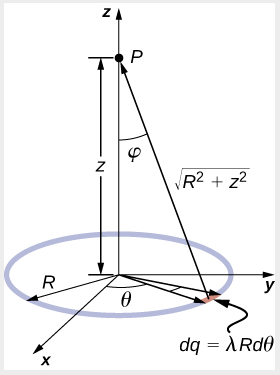
\includegraphics[width=0.22\textwidth]{ring.png}
\caption{\label{fig:ring} A ring of charge situated in the xy-plane.}
\end{figure}
\item As $z \rightarrow \infty$ in Fig. \ref{fig:ring}, what happens to the field?
\begin{itemize}
\item A: The field-strength increases.
\item B: The field-strength remains constant.
\item C: The field-strength decreases.
\item D: The field-strength is exactly zero.
\end{itemize}
\item Suppose the actual function for the E-field $\vec{E}(z)$ is
\begin{equation}
\vec{E}(z) = \frac{1}{4\pi \epsilon_0} \frac{q z}{\left( z^2 + R^2 \right)^{3/2}} \hat{z} \label{eq:eq1}
\end{equation}
To see what happens when $z$ is much larger than $R$, try setting $R=0$.  What is the result in Eq. \ref{eq:eq1} if $R=0$? \\ \vspace{1cm}
\item Do you recognize the expression?  What does the ring resemble if $R \approx 0$?
\item \begin{figure}[ht]
\centering
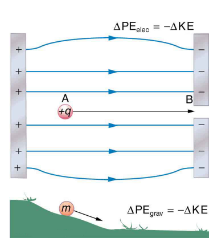
\includegraphics[width=0.22\textwidth]{hill.png}
\caption{\label{fig:hill} The relationship between potential energy and voltage.}
\end{figure}
Consider Fig. \ref{fig:hill}.  Suppose the mass $m$ rolls down a hill from a height of 30 meters.  In the absense of \textit{friction}, what will be the final speed of the object? \\ \vspace{1cm}
\item Consider Fig. \ref{fig:hill}.  Suppose the charge is $q = 1 \mu$C, and the voltage is 12 V.  (a) What is the potential energy before the charge is released? (b) If the charge has a mass of $10^{-6}$ kg, what will the final speed be after the charge is released? \\ \vspace{1.0cm}
\item Suppose two parallel plate capacitors are added in parallel.  One has an area of 1.0 mm$^2$, and a plate separation of 0.1 mm, and the other has area 0.5 mm$^2$ and separation 0.2 mm.  What is the total capacitance of the system? \\ \vspace{1cm}
\item 
\begin{figure}
\centering
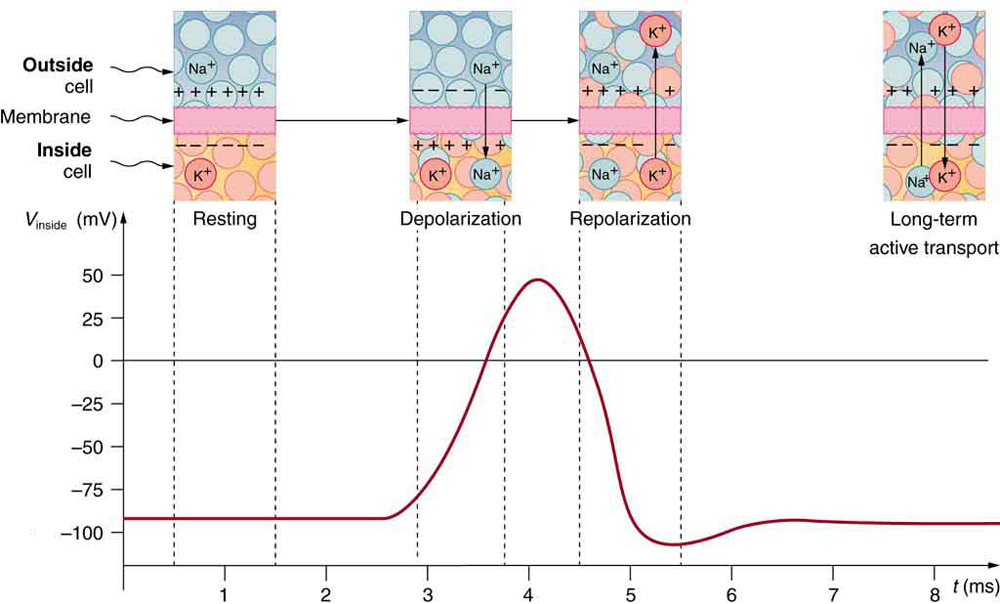
\includegraphics[width=0.5\textwidth]{nerve.jpeg}
\caption{\label{fig:nerve} A nerve signal in the human body.}
\end{figure}
Suppose an ion with the charge of an electron is accelerated by the positive 50 mV of the nerve signal potential shown in Fig. \ref{fig:nerve} for 1 ms.  (a) What is the final energy of the ion?  (b) What current does this represent?  (c) Suppose there are $10^{23}$ ions moving in the same way.  What current does this represent? (d) Suppose the cell wall is 50 nm thick.  What is the electric field across it, if the potential difference is the maximum in Fig. \ref{fig:nerve} minus the minumum in Fig. \ref{fig:nerve}? \\ \vspace{3cm}
\item (a) What is the power consumption of a 24 V system that draws 0.5 A of current? (b) If a different system operates at 12 V, and has a total resistance of 50$\Omega$, what is the power consumption? \\ \vspace{1cm}
\item Suppose a a battery is connceted in series with a resistor.  The $\epsilon$, or emf of the battery is 14 V and the resistance is 50$\Omega$.  The current is measured to be 266 mA.  What is the \textit{internal resistance} of the battery? \\ \vspace{1.5cm}
\item Consider Fig. \ref{fig:lorentz}, in which a DC power generator is depicted inside a 0.05 T B-field.  Suppose the area of the loop is $10^{-2}$ m$^{2}$, the voltage in the circuit is 24 V, and the circuit resistance is 50 $\Omega$.  Also assume that there is just one loop of wire in the rotor.  What is the \textit{maximum torque} the system could achieve? \\ \vspace{2cm}
\begin{figure}[ht]
\centering
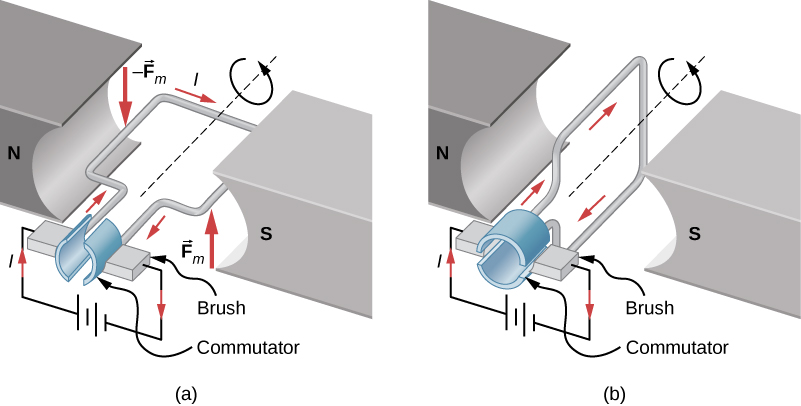
\includegraphics[width=0.55\textwidth]{commute.jpeg}
\caption{\label{fig:lorentz} An illustration of how a power generator works.  This version uses DC current and a commutator.}
\end{figure}
\item What would the maximum torque be if there were $N = 100$ turns of wire? \\ \vspace{1cm}
\item Consider Fig. \ref{fig:acgen}.  Suppose that the angle between the area vector and the magnetic field is $\theta = \omega t$.  (a) Show that
\begin{equation}
\phi(t) = BA\cos(\omega t) \label{eq:ac}
\end{equation}
(b) Given Eq. \ref{eq:ac}, it turns out that the voltage generated in the loop is proportional to $\sin(\omega t)$ and $\omega$ itself.  That is,
\begin{equation}
\epsilon(t) = BA\omega \sin(\omega t)
\end{equation}
What is the voltage at a time $t = 1/240$ seconds, $\omega = 120\pi$ Hz, $B = 0.1$ T, and $A = 0.01$ m$^2$? (c) At what time is the voltage zero? \\ \vspace{3cm}
\begin{figure}[hb]
\centering
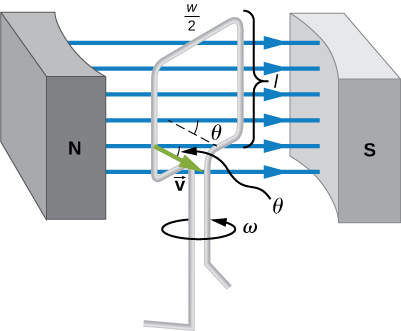
\includegraphics[width=0.35\textwidth]{acGen.jpeg}
\caption{\label{fig:acgen} A schematic of the concept of an AC generator.}
\end{figure}
\item Suppose the AC generator in Fig. \ref{eq:ac} has $V_0 = 12$ V so that $\epsilon(t) = V_0 \sin(\omega t)$.  If the AC generator pushes current through a resistance $R = 50\Omega$, what is the average power generated?
\end{enumerate}

\end{document}